\begin{frame}{Reality check}
  \pause
  \begin{center}
    \large
    Most of the code we write is \\ \textbf{ill-typed}
  \end{center}

  \note[item]{And maybe it's when we might be dozing off from the great lunch on Friday afternoon
    that we need a reality check}
  \note[item]{And the reality is that most of the code we write is ill-typed}
  \note[item]{In fact, most of the time, we're still in the midst of typing out the darn thing, so
    naturally it's probably very ill-typed indeed}
  \note[item]{Or think about that time you changed an important data type or function signature and
    spent the next several hours or days fixing the rest of your code---these ill-typed states can
    persist for a long time}
\end{frame}

\begin{frame}{Localization and recovery}
  As programmers, we want tooling can \\[1em]

  \pause
  \begin{itemize}
    \item \textbf{localize type errors}\pause: describe \emph{what} and \emph{where} they are

      \pause
    \item \textbf{recover}: even when an error is encountered,
      continue to provision downstream services and find other errors
  \end{itemize}

  \vspace{1em}
  \ie, code completion, type hints, and other downstream services shouldn't suddenly all fail
  because of one error!

  \note[item]{For these reasons we hope, or rather expect, our editor services and tooling to be
    able to cope with our ill-typed code}
  \note[item]{In particular that means we expect them to}
  \note[item]{first of all, localize type errors, or tell us what and where they are in our code}
  \note[item]{and, even in the face of errors, recover optimistically to continue doing what it's
    doing and find other errors, ideally with minimal loss in service}
  \note[item]{Naturally, this problem has garnered plenty of practical interest, and we can see
    that production tooling supports some form of localization and recovery capability.}
\end{frame}

\newcommand<>{\localized}[1]{\alt#2{\fboxsep=2pt\samesizecolorbox{Red!30}{$#1$}}{#1}}
\newcommand<>{\localizedAux}[1]{\alt#2{\fboxsep=2pt\samesizecolorbox{Emerald!30}{$#1$}}{#1}}

\begin{frame}[fragile, t]
  \frametitle<1-3>{Observations in practice}
  \frametitle<4-5>{OCaml: the first branch is right}
  \frametitle<6>{Haskell: 5 is the problem}
  \frametitle<7>{Rust: maybe 5 is also the problem?}
  \frametitle<8>{Hazel: the whole thing's all messed up!}

  \begin{center}
    $%
      \ELet{f}{\ELam{b}{\TBool}{\cdots}}{\pause
        \ELet{x}
          {\localized<8>{\EIf{\ETrue}
               {\localizedAux<7>{\localized<6>{\ENum{5}}}}
               {\localized<4-5,7>{\EFalse}}}}
          {\pause\EAp{f}{\localized<5>{x}}}
      }
    $%
  \end{center}
  %
  \begin{semiverbatim}\small\only<4-5>{
1 | let x = if true then 5 else \textcolor{red}{\textbf{false}} in f x
                                \textcolor{red}{^^^^^}
\textcolor{red}{\textbf{Error}}: This expression \textbf{has type bool} but an expression
         was \textbf{expected of type int}
     \only<5>{
1 | let x = if true then 5 else false in f \textcolor{red}{\textbf{x}}
                                           \textcolor{red}{^}
\textcolor{red}{\textbf{Error}}: This expression \textbf{has type int} but an expression
         was \textbf{expected of type bool}}}\only<6>{
Main.hs:4:26: \textbf{\textcolor{red}{error}:} [GHC-39999]
    • \textbf{No instance for ‘Num Bool’ arising from the literal ‘5’}
  |
4 | _ = let x = if True then \textcolor{red}{\textbf{5}} else False in f x
  |                          \textcolor{red}{\textbf{^}}}\only<7>{
\textbf{\textcolor{red}{error[E0308]}: `if` and `else` have incompatible types}
 --> src/main.rs:2:30
  |
6 | let x = if true { 5 } else { false }; f(x);
  |                  \textcolor{Emerald}{\textbf{-}}        \textcolor{red}{\textbf{^^^^^ expected integer, found `bool`}}
  |                  \textcolor{Emerald}{\textbf{|}}
  |                  \textcolor{Emerald}{\textbf{expected because of this}}}
  \end{semiverbatim}

  \only<8>{
    \begin{center}
      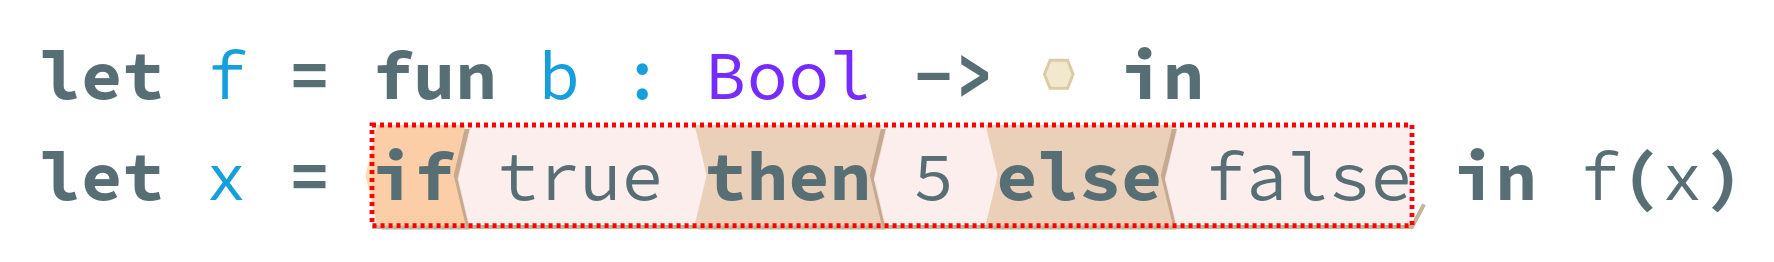
\includegraphics[width=0.9\linewidth]{media/inconsistent.png}
      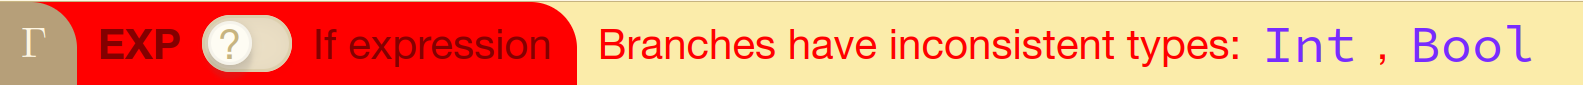
\includegraphics[width=0.9\linewidth]{media/inconsistent-ci.png}
    \end{center}
  }

  \note[item]<1-3>{Let's look for example at this program, in which we've a function f that takes a
    boolean---and does something}
  \note[item]<1-3>{x is determined by a conditional}
  \note[item]<1-3>{and f is applied to x}
  \note[item]<1-3>{We can immediately see that the branches of the conditional are mismatched wrt to
    typing, so there should be some sort of error diagnostic}
  \note[item]<4->{and in fact if we throw this at the OCaml compiler, it says, yes, there is, and it's
    on the false, having prioritized the first branch's integer}
  \note[item]<4->{ocamlc will stop here, but merlin, which powers editor services nowadays, will also
    say that there's another error on the usage of x, since it's determined x to be an int but f takes
    a bool}
  \note[item]<4->{OK, that's all well and good, so what about Haskell?}
  \note[item]<4->{Somewhat unexpectedly, it localizes the error to 5, complaining that it isn't an
    instance of Num Bool---this is presumably because of how type inference works for the Num type
    class}
  \note[item]<4->{Rust is a little different in that it prioritizes the first branch like OCaml but
    also suggests that the 5 is to blame}
  \note[item]<4->{Hazel, the programming environment our group is building, is still different,
    assigning the error to the entire conditional with the cursor inspector stating that the
    branches are inconsistent}
\end{frame}

\begin{frame}{Observations in practice}
  Today's tooling is error-resilient to a certain degree\pause, but \\[1em]

  \pause
  \begin{itemize}
    \item localization can be varied\pause, often guessing about \emph{user intent}

      \pause
    \item recovery necessitates reasoning without complete knowledge about types

      \pause
    \item decisions can influence other downstream decisions
  \end{itemize}

  \note[item]{Now obviously these languages all have different kinds of type systems, but from this
    informal exercise we can observe that practical systems are type error-resilient to a
    certain degree}
  \note[item]{but}
  \note[item]{decisions about how to localize can vary, and often tools will try to guess users'
    intentions about where to localize errors to}
  \note[item]{Then, to recover, they have to somehow operate with incomplete knowledge about the
    types at play}
  \note[item]{and together, upstream error localization decisions, once recovered from, can
    influence downstream decisions, sometimes unexpectedly}
  \note[item]{We think, therefore, that this subject would benefit greatly from rigorous treatment}
  \note[item]{Unfortunately, our current developments in theory don't reflect this reality}
\end{frame}

\begin{frame}{A definitional gap problem}
  \begin{center}
    Most of the code we write is \emph{ill-typed}\pause,
    but conventional language definitions
    \emph{only specify the behaviour of well-typed programs}. \\[0.5em]

    \pause
    $\Gamma \vdash e : \tau$
  \end{center}
  \pause
  \[%
    \bm{\Downarrow}
  \]%

  \begin{center}
    If a type error appears \textcolor{RedOrange}{\textbf{anywhere}},\\
    the program is meaningless \textcolor{Red}{\textbf{everywhere}}.
  \end{center}

  \note[item]{Most of the code we write is ill-typed, but conventional language definitions are only
    concerned with the semantics of well-typed programs}
  \note[item]{This is made most obvious by the fact that our type systems look generally like some
    variation of this judgment form}
  \note[item]{So if a type error appears anywhere}
  \note[item]{as far as the specification are concerned, the program becomes meaningless as a whole}
\end{frame}

\begin{frame}{The goal}
  We'd like a way to formally specify type checkers that are capable of localizing and recovering
  from errors \\[1em]

  \pause
  \begin{emphbox}{Totality}
    These semantics should describe \emph{both well-typed and ill-typed programs}.
  \end{emphbox}

  \note[item]{We'd like a way to alleviate this, by being able to create precise specifications for
    the typing semantics of these ill-typed programs, localizing and recovering from type errors along
    the way}
  \note[item]{And these type checker semantics should describe both well-typed and ill-typed
    programs}
  \note[item]{This notion we'll call totality, and it'll serve as a sort of guiding principle}
\end{frame}

\begin{frame}{This paper is about\ldots}
  \pause
  Uniting \emph{local} and \emph{global} type inference for principled total type error localization and
  recovery: \\[1em]

  \begin{itemize}
    \item<3-> the \textbf{marked lambda calculus}%
      \uncover<4->{%
        : a judgmental framework for bidirectional type error localization and recovery%
      }

    \item<5-> \textbf{type hole inference}%
      \uncover<6->{%
        : a global, constraint-based system \\
        that is neutral in error localization and recovery
      }
  \end{itemize}

  \note[item]{In this work, we've developed techniques to achieve total type error localization and
    recovery}
  \note[item]{by elegantly blending local and global type inference}
  \note[item]{For the former, we present in tutorial-style the marked lambda calculus}
  \note[item]{a judgmental framework for type error localization and recovery for bidirectional type
    systems}
  \note[item]{We choose bidirectional systems as our starting point because it creates a flow of
    typing data that is conducive to intuitive error localization}
  \note[item]{Then, we'll describe type hole inference, or how to layer a global constraint-based
    inference system atop the marked lambda calculus in a way that allows us to neatly combine the
    bidirectional and unification approaches for even better localization}
  \note[item]{While these two paradigms have been often thought of as opposing or alternative
    techniques, in this talk we'll hopefully see how they supplement each other}
\end{frame}
